\chapter{Implementing Internal Model Controller for First Order System on a Single Board Heater System}
This experiment aims to implement an Internal Model Controller for first order systems on a Single Board Heater System. 
The target group is anyone possessing basic knowledge of control engineering.\\
\begin{figure}
	\centering
		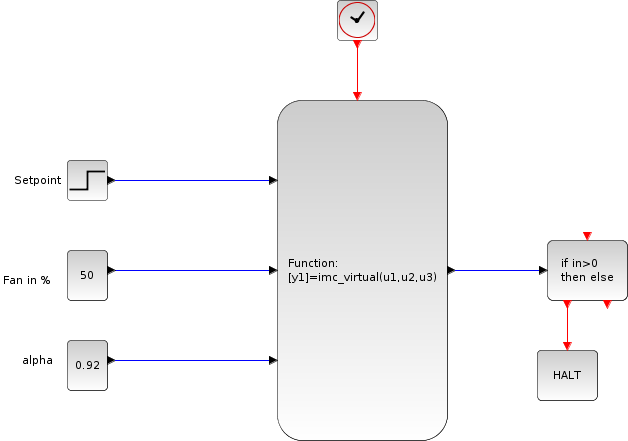
\includegraphics[width=\linewidth]{IMC/imc_virtual_xcos.png}
	\caption{Xcos interface for this experiment}
	\label{Xcos_imc}
\end{figure}
Scilab is used with Xcos as an interface for sending and receiving data. 
This interface is shown in figure \ref{Xcos_imc}. Fan speed and heater current are the two inputs to the system. 
For this experiment, the heater current is the control effort or manipulated variable. 
The fan input is considered to be the external disturbance.

\section{IMC Design for Single Board Heater System}
Internal Model Controller contains explicit model of plant \cite{kmmdc09}. 
The closed loop system can be stabilized with the use of a stable open loop transfer function and a stable controller. 
The IMC is mainly used for stable plants.\\
\begin{figure}
\begin{center}
\begin{tikzpicture}[auto,node distance=2cm]
\node[input](input){};
\node[sum,right of=input](sum1){};
\draw[->](input)--node{$r$}(sum1);
\node[block,right of=sum1](gqz){$G_Q(z)$};
\draw[->](sum1)--node{$e$}(gqz);
\node[branch,right of=gqz, node distance=2cm](b1){};
\node[block, right of=b1](gpz){$G_p(z)$};
\draw[->](gqz)--node{$u$}(gpz);
\node[sum, right of=gpz,pin={[pinstyle] above:$\xi$},node distance=2cm](sum2){};
\draw[->](gpz)--(sum2);
\node[output, right of=sum2](output){};
\draw[->](sum2)--node{$y$}(output);
\node[branch, right of=sum2, node distance=1cm](b2){};
\node[sum, below of=b2,node distance=2cm](sum3){};
\draw[->](b2)--(sum3);
\node[block,below of=gpz](gz){$G(z)$};
\draw[->](b1)|-(gz);
\draw[->](gz)--node{$\bar{y}$\hspace{0.7cm} $-$}(sum3);
\draw[->](sum3)--(10,-3)-|node[pos=0.88]{$-$}(sum1);
\end{tikzpicture}
\end{center}
\caption{IMC feedback configuration}
\label{imcfeedback}
\end{figure}

Let the transfer function of the stable plant be denoted by $G_p (z)$ and its model is denoted by $G(z)$. Hence
\begin{align}
y(n) = G(z)u(n)+\xi(n) 
\end{align}
where: \\
y(n) = plant output\\
      u(n) = plant input\\
      $\xi$(n) = noise
      
% Figure \ref{imcfeedback} shows method to control stable plant by using internal model control.
For noise rejection with y=0, we require $G_Q=G_p^{-1}$ and $G=G_p$, i.e., for stable $G_Q$ we require 
an approximate inverse of G. Also, for internal stability, transfer function between any two points 
in the feedback loop must be stable \cite{kmmdc09}.
\begin{figure}
\begin{center}
\begin{tikzpicture}[auto,node distance=2cm]
\node[input](input){};
\node[sum,right of=input](sum1){};
\draw[->](input)--node{$r$}(sum1);
\node[sum, right of=sum1](sum2){};
\draw[->](sum1)--(sum2);
\node[block,right of=sum2](gqz){$G_Q(z)$};
\draw[->](sum2)--node{$e$}(gqz);
\node[branch,right of=gqz, node distance=2cm](b1){};
\node[block, right of=b1](gpz){$G_p(z)$};
\draw[->](gqz)--node{$u$}(gpz);
\node[sum, right of=gpz,pin={[pinstyle] above:$\xi$},node distance=2cm](sum3){};
\draw[->](gpz)--(sum3);
\node[output, right of=sum3](output){};
\draw[->](sum3)--node{$y$}(output);
\node[block, below of=gqz](gz){$G(z)$};
\draw[->](b1)|-(gz);
\draw[->](gz)-|(sum2);
\draw[->](sum3)--(10,-3)-|node[pos=0.88]{$\bar{\xi}$}(sum1);
\end{tikzpicture}
\end{center}
\caption{IMC feedback configuration}
\label{feedback}
\end{figure}

\section{Step for Designing IMC for Stable Plant}
IMC design refers to obtaining a realizable $G_Q$ that is stable and approximately inverse of G. 
This can be achieved by inverting the delay free plant model so that $G_Q$ is realizable. 
For non-minimum phase part of the plant, reciprocal polynomial is used for stable controller. 
Negative real part of the plant should be replaced with the steady state equivalent of that part to avoid oscillatory 
nature of control effort. Low pass filter must be used to avoid the high frequency components because of the model mismatch.
The SBHS is modeled as-
\begin{align}
	G&=Z^{-1} \frac{0.01163}{1-0.9723Z^{-1}}
\intertext{Inverting delay free plant, we get}
\frac{A}{B}&=\frac{1-0.9723Z^{-1}}{0.01163}
\intertext{Comparing plant model with equation}
G&=Z^{{-1}}\frac{B^g B^- B^{nm+}}{A}\\
\intertext{We get,}
B^g&=0.01163\\
B^-&=1\\
B^{nm+}&=1\\
A&=1-0.9723Z^{-1}
\intertext{For the stable system, internal model controller is given by}
G_Q&=\frac{A}{B^gB^-_s B_r^{nm+}}G_f\\
G_Q&=\frac{1-0.9723Z^{-1}}{0.01163}\frac{1-\alpha}{1-\alpha Z^{-1}}
\intertext{Now,}
G_c&=\frac{G_Q}{1-GG_Q}\\
\frac{u}{e}&=\frac{\frac{1-0.9723Z^{-1}}{0.01163}\frac{1-\alpha}{1-\alpha Z^{-1}}}{1-Z^{-1}\frac{0.01163}{1-0.9723Z^{-1}}\frac{1-0.9723Z^{-1}}{0.01163}\frac{1-\alpha}{1-\alpha Z^{-1}}}\\
\intertext{After simplifying, we get}
\frac{u}{e}&=\frac{1-\alpha}{0.01163}\frac{1-0.9723Z^{-1}}{1-Z^{-1}}\\
\frac{u}{e}&=b\frac{1-0.9723Z^{-1}}{1-Z^{-1}}
\intertext{where,}
b&=\frac{1-\alpha}{0.01163}
\intertext{Hence,}
u(n)&=u(n-1)+b[e(n)-0.9723e(n-1)]
\end{align}


The output of Xcos is shown in figure \ref{imc}.
Figure shows three plots. First sub plot shows setpoint and output temperature profile. 
Second sub plot shows control effort and third sub plot shows error between setpoint and plant output.




\begin{figure}
	\centering
		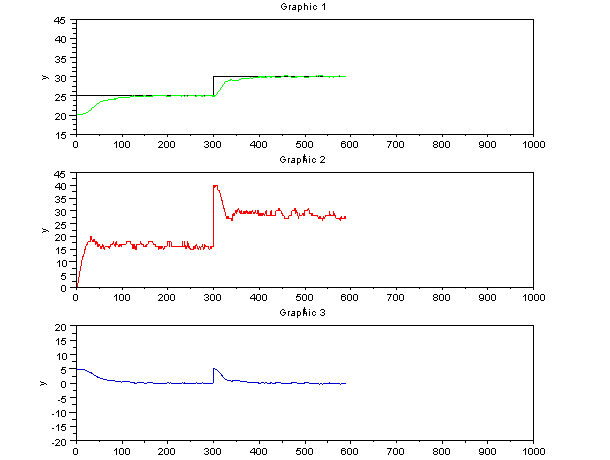
\includegraphics[width=\linewidth]{IMC/imc_092_resp.png}
	\caption{Experimental results with IMC for $\alpha=0.92$}
	\label{imc}
\end{figure}
\begin{figure}
	\centering
		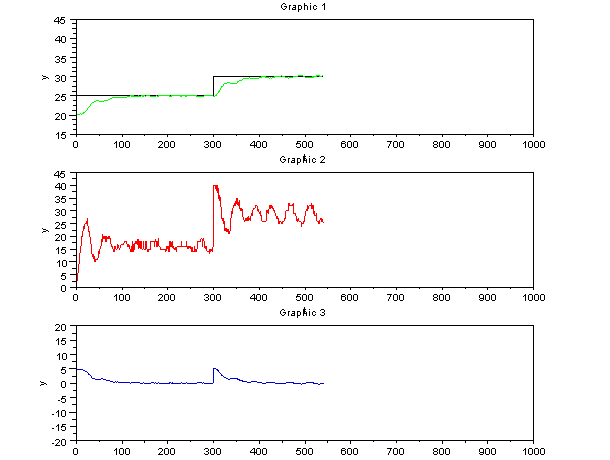
\includegraphics[width=\linewidth]{IMC/imc_085_resp.png}
		\caption{Experimental results with IMC for $\alpha=0.85$}
	\label{fig:0.85}
\end{figure}

The same experiment result for $\alpha=0.85$ is as shown in fig \ref{fig:0.85}.
By comparing the two graphs, we can say that for $\alpha=0.92$ the response of the controller is sluggish. For $\alpha=0.85$,
the controller starts responding quickly and no overshoots are seen in the temperature profile.

\subsection{Implementing IMC locally}
The detailed procedure to perform a local experiment is explained in Chapter\ref{sercomm}. A summary of the same is provided in section \ref{local-summary} It is same for this section with following changes.

\begin{enumerate}
\item Step1: The working directory is {\tt  imc\_controller}
\item Step2: Same
\item Step3: Same
\item Step4: Same
\item Step5: Load ramp test function by executing command\\ {\tt exec<space>imc.sci}
\item Step6: Load Xcos code for ramp test using the command\\ {\tt exec<space>imc.xcos}
\item Step7: Same
\end{enumerate}

\subsection{Implementing IMC virtually}

The detailed procedure to perform a virtual experiment is explained in Chapter\ref{virtual}. A summary of the same is provided in section \ref{vlabsexpt}. It is same for this section with following changes.

\begin{enumerate}
\item Step1: The working directory is {\tt  imc\_controller}. Open this directory.
\item Step2: Same
\item Step3: Same
\item Step4:  Switch to the IMC  experiment directory and double-click on the file {\tt imc.sce}. This will launch scilab and also open the file {\tt imc.sce} in the scilab editor. Linux users will have to launch scilab manually. They also have to change the working directory to {\tt imc\_controller} and then open the {\tt  imc.sce} file in the scilab editor.
\item Step5: Same
\item Step6: Execute the file {\tt imc.sce}.  Expect the IMC controller xcos diagram to open automatically. If this doesnt happen, check the scilab console for error message.
\item Step7: Execute the IMC controller xcos diagram.
\item Step8: Same
\end{enumerate}


\section{Scilab Code}\label{imccodes}
\begin{code}
\ccaption{ser\_init.sce}{\ttfamily ser\_init.sce}
\lstinputlisting{Scilab/local/imc_controller/ser_init.sce}
\end{code}

\begin{code}
 \ccaption{imc.sci}{\ttfamily imc.sci}
\lstinputlisting{Scilab/local/imc_controller/imc.sci}
\end{code}


\begin{code}
 \ccaption{imc\_virtual.sce}{\ttfamily imc\_virtual.sce}
\lstinputlisting{Scilab/virtual/imc_controller/imc_virtual.sce}
\end{code}


\begin{code}
 \ccaption{imc\_virtual.sci}{\ttfamily imc\_virtual.sci}
\lstinputlisting{Scilab/virtual/imc_controller/imc_virtual.sci}
\end{code}


%\bibliography{imc} 
